\clearpage
\appendix
\section*{Anexos}
\subsection*{Anexo A. Código y reproducibilidad}
Los archivos de implementación (\texttt{.m} y \texttt{.mlx}), las figuras y las tablas de resultados están en el repositorio del proyecto: \url{https://github.com/jmtimana/CC2104-UMZ-SIRS-Grupo8}. Cada experimento se ejecuta de forma independiente desde la carpeta de código y escribe sus resultados en \texttt{resultados/} y sus figuras en \texttt{figuras/}.

\subsection*{Anexo B. Matriz jacobiana por bloques}\label{anx:jacobiana}
Con $\bar b_2'(I)=Kb_2/(1-KI)^2$, $\partial_M\bar\beta=\beta/(1+Z)$ y $\partial_Z\bar\beta=-\beta(1+M)/(1+Z)^2$, la jacobiana $\mathbf J_f=\begin{pmatrix}\mathbf J_{ff}&\mathbf J_{fs}\\ \varepsilon\mathbf J_{sf}&\varepsilon\mathbf J_{ss}\end{pmatrix}$ tiene los bloques
\begin{align*}
\mathbf J_{ff}&=\begin{pmatrix}-(b_1M+\bar b_2Z+\mu_1)&-b_1U&-\bar b_2U\\ b_1M&b_1U-\mu_1&0\\ \bar b_2Z&0&\bar b_2U-\mu_1\end{pmatrix},\\
\mathbf J_{fs}&=\begin{pmatrix}0&-\bar b_2'UZ&0\\0&0&0\\0&\bar b_2'UZ&0\end{pmatrix},\\
\mathbf J_{sf}&=\begin{pmatrix}0&-SI\,\partial_M\bar\beta&-SI\,\partial_Z\bar\beta\\0&SI\,\partial_M\bar\beta&SI\,\partial_Z\bar\beta\\0&0&0\end{pmatrix},\\
\mathbf J_{ss}&=\begin{pmatrix}-(\bar\beta I+\mu_2)&-\bar\beta S&\eta\\ \bar\beta I&\bar\beta S-\gamma-\mu_2&0\\0&\gamma&-(\eta+\mu_2)\end{pmatrix}.
\end{align*}
Los bloques $\mathbf J_{fs}$ y $\mathbf J_{sf}$ contienen las únicas derivadas cruzadas y materializan el acoplamiento entre capas.

\subsection*{Anexo C. Adaptación del paso}\label{anx:pasos}
\begin{figure}[h]
\centering
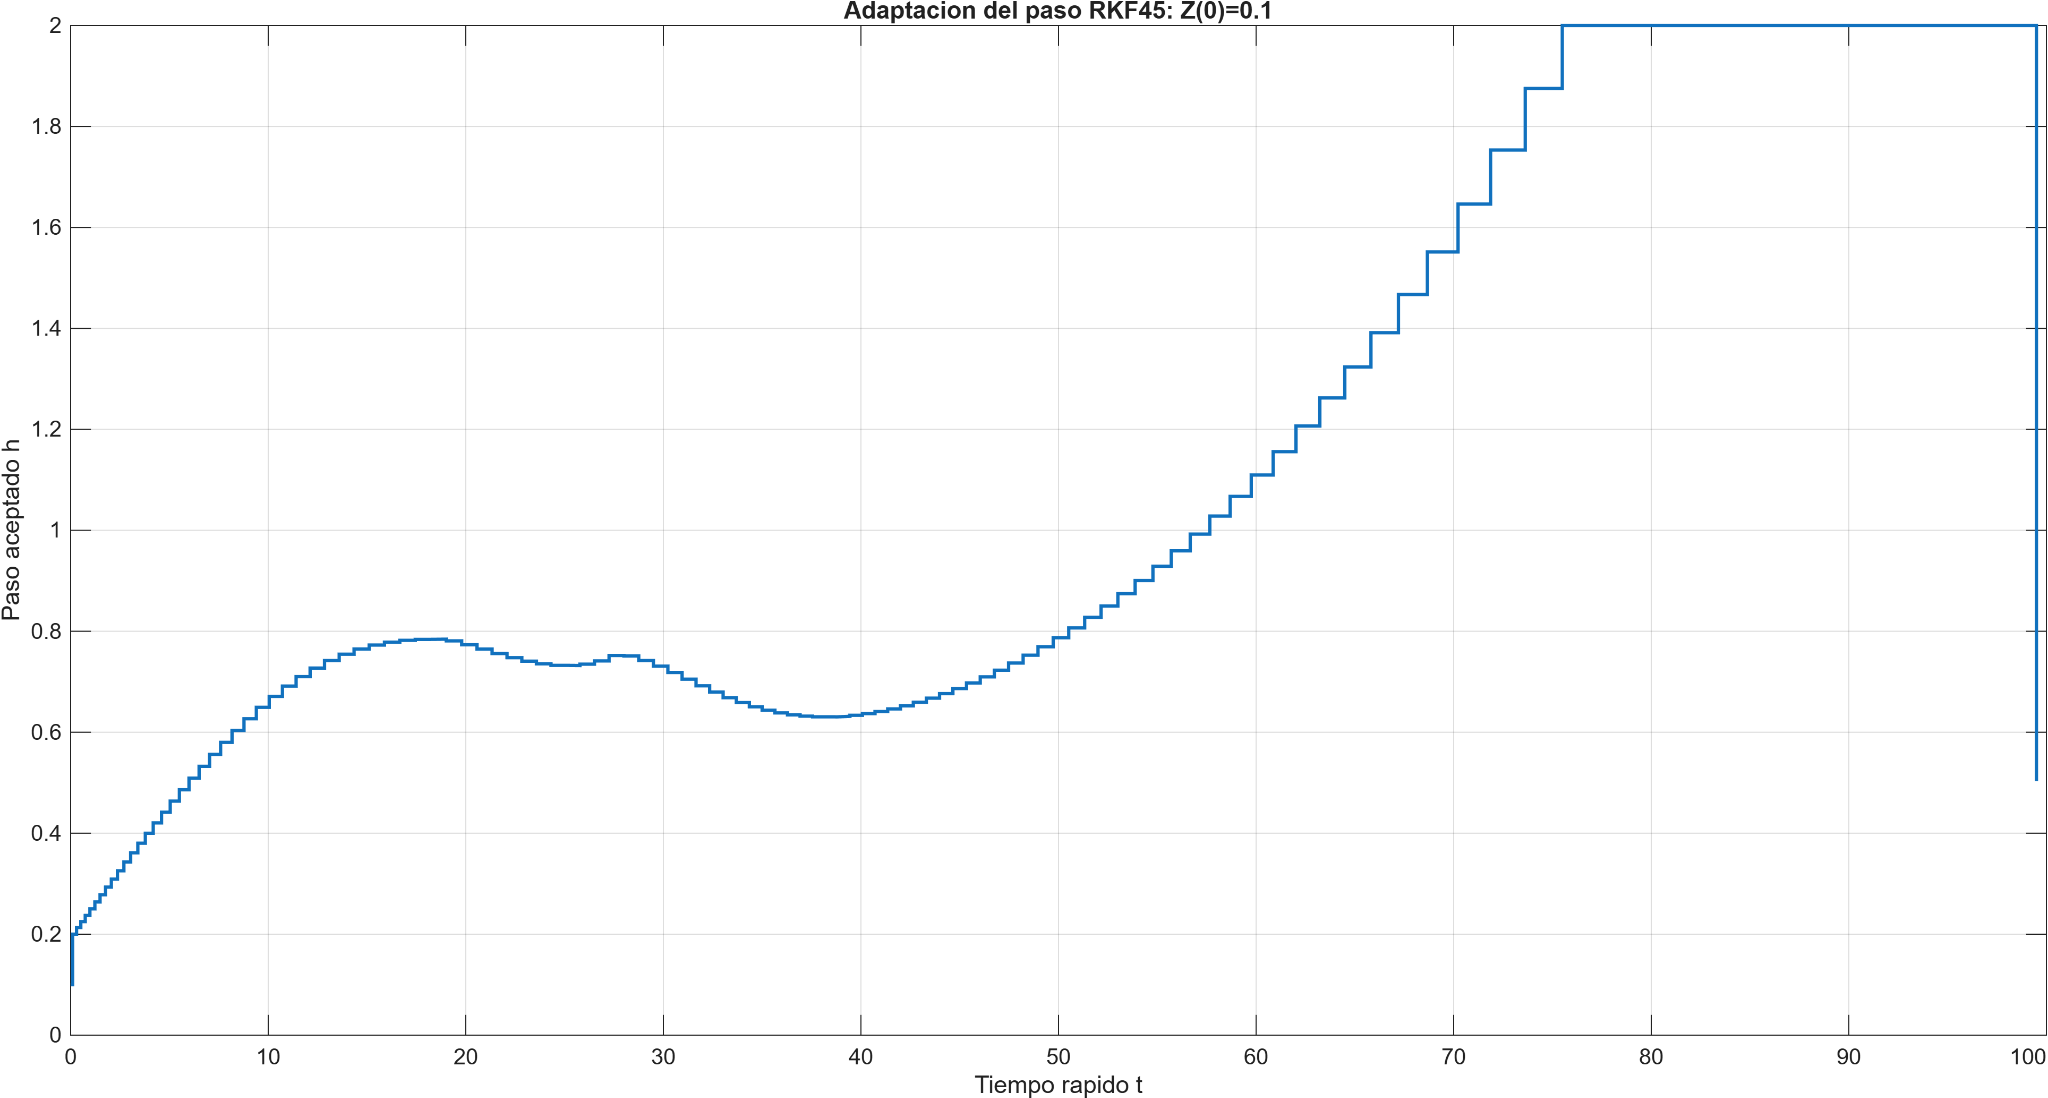
\includegraphics[width=\columnwidth]{imagenes/fig05_paso_adaptativo_rkf45.png}
\caption{Paso aceptado por RKF45 ($\varepsilon=0.01$, $r_{\rm tol}=10^{-8}$, $Z(0)=0.1$). La meseta en $h=2$ corresponde al tope $h_{\max}$; no hubo pasos rechazados.}
\label{fig:rkf45}
\end{figure}

\begin{figure}[h]
\centering
\includegraphics[width=\columnwidth]{imagenes/fig09_paso_efectivo.png}
\caption{Paso aceptado durante la integración ($\varepsilon=0.01$, $h$ nominal $=4$, con reducción de paso y RKF45 adaptativo).}
\label{fig:paso}
\end{figure}
